\documentclass[10pt,twocolumn,letterpaper]{article}

% Margini da conferenza: i margini di default di article su letterpaper
% lasciano una cornice bianca che su due colonne costa quasi un terzo
% della pagina.
\usepackage[letterpaper,margin=0.75in,columnsep=0.25in]{geometry}

\usepackage{graphicx}
\usepackage{amsmath,amssymb}
\usepackage{booktabs}
\usepackage{multirow}
% hidelinks: senza cvpr.sty hyperref disegna un riquadro attorno a
% ogni \ref e \cite.  Lo togliamo, i link restano cliccabili.
\usepackage[hidelinks]{hyperref}
\usepackage{xcolor}

% Le figure stanno in <repo>/plots, questo file in <repo>/paper
\graphicspath{{../}}

% La figura qualitativa a piena pagina supera i limiti di default per i
% float a due colonne e finirebbe dopo la bibliografia.
\renewcommand{\dbltopfraction}{0.9}
\renewcommand{\dblfloatpagefraction}{0.7}

% Convenience
\newcommand{\eg}{\emph{e.g.}}
\newcommand{\ie}{\emph{i.e.}}
\newcommand{\etal}{\emph{et al.}}

% Limite: 8 pagine escluse le references.

\title{Beyond Single Prompts: Comparing Vision Adapters, CoOp,\\
and Optimal Transport for Domain-Specific Image Classification}

\author{
  Mattia Lomuto (VR543327)
  \and Carlo Stasi (VR543606)
  \and Marco Equisetto (VR535007)
  \\[4pt]
  \textit{Advanced Programming for AI}\\
  \textit{University of Verona}\\
  {\small\texttt{\{mattia.lomuto, carlo.stasi, marco.equisetto\}@studenti.univr.it}}
}
\date{}

% Senza raggedbottom, in una colonna accanto ai float LaTeX distribuisce
% lo spazio avanzato fra i paragrafi.
\raggedbottom

\begin{document}
\maketitle

\begin{abstract}
While vision--language models like CLIP offer strong zero-shot transfer,
they often struggle on specialized visual domains.  To measure how much
accuracy each trainable parameter buys, we compare seven adaptation
strategies (including CoOp, CLIP-Adapter, Tip-Adapter and LoRA) against
zero-shot baselines on a single frozen CLIP ViT-B/32 backbone, with one
few-shot protocol, evaluation loop and epoch budget across EuroSAT, DTD
and Flowers102, and report accuracy alongside parameter count, GPU memory
and training time.  Much of the gain comes from the labelled support
images rather than from the parameters that exploit them: on EuroSAT a
linear probe and the training-free Tip-Adapter already close 82\,\% and
70\,\% of the gap between zero-shot CLIP and the best adapted model.  On
DTD and Flowers102, where those two close at most 69\,\%, CoOp's
8{,}192 context parameters (0.005\,\% of the backbone) close 90\,\% and
76\,\% of it, while Tip-Adapter-F reaches the highest accuracy on two of
the three datasets.

\smallskip\noindent\textbf{Code:}~\url{https://github.com/MarcoEquisetto/APAI_exam}
\end{abstract}


\section{Introduction}\label{sec:introduction}

Contrastive Language--Image Pre-training (CLIP)~\cite{radford2021learning}
aligns images and captions in a shared embedding space and classifies
images through natural-language prompts, without task-specific training.
In specialised domains, however, zero-shot accuracy remains far from
satisfactory: a frozen ViT-B/32 reaches only 46.4\,\% on
EuroSAT~\cite{helber2019eurosat}, 54.9\,\% on
DTD~\cite{cimpoi2014describing} and 71.5\,\% on
Flowers102~\cite{nilsback2008automated}.  Fine-tuning all 151~million
parameters requires large labelled datasets and risks catastrophic
forgetting of the visual--linguistic knowledge that makes CLIP useful.
\emph{Parameter-efficient adaptation} instead trains a small number of new
parameters on top of the frozen backbone.  Methods differ in \emph{where}
they intervene and in \emph{how many parameters} they introduce, from zero
(training-free caches) to several hundred thousand (LoRA inside the
backbone).

\paragraph{Prior work.}
\textbf{CoOp}~\cite{zhou2022learning} replaces the hand-written prompt
template with $M$ learned context vectors.
\textbf{CLIP-Adapter}~\cite{gao2024clipadapter} appends a residual
bottleneck MLP to the frozen visual encoder.
\textbf{Tip-Adapter}~\cite{zhang2022tip} builds a training-free key--value
cache from the support images, and \textbf{Tip-Adapter-F} fine-tunes its
keys.  \textbf{LoRA}~\cite{hu2022lora} injects low-rank updates into
existing linear layers, adapting \emph{inside} the backbone.  Finally,
\textbf{Optimal Transport}~\cite{cuturi2013sinkhorn} compares distributions
of patch and word tokens through the Sinkhorn distance.  These results are
hard to compare with one another: backbones, shot counts, sampling seeds
and training schedules vary from paper to paper.  Efficiency is rarely
tabulated---GPU memory, training time and trainable parameters are seldom
measured on the same hardware---and negative results, na\"ive token-level
Optimal Transport among them, largely go unpublished.

\paragraph{Contributions.}
We implement ten methods in a \textbf{single codebase} sharing one frozen
ViT-B/32 backbone (LAION-2B weights via OpenCLIP), one evaluation loop,
one few-shot sampler and one epoch budget, so that accuracy, parameter
count, GPU memory and wall-clock time are directly comparable.  We
quantify the \textbf{accuracy per trainable parameter} on three domains
and find that the labelled support set, more than the parameter count,
drives accuracy: the best method with fewer than 10{,}000 trainable
parameters closes 76--90\,\% of the gap between zero-shot CLIP and the
best method in our grid.  We build a \textbf{joint CoOp\,+\,CLIP-Adapter}
model and document what composing two independently developed modules
requires---MRO conflicts, optimiser recipes, gradient-flow traps.  We also
report an \textbf{informative negative result}, analysing why Sinkhorn
Optimal Transport on patch tokens fails to beat zero-shot CLIP.


\section{Method}\label{sec:method}

\subsection{Frozen Backbone and Shared Interface}\label{sec:backbone}

All experiments use an OpenCLIP ViT-B/32 with LAION-2B weights
(\texttt{laion2b\_s34b\_b79k}): a 12-layer vision transformer (about
88\,M parameters) and a 12-layer text transformer (about 63\,M), 151\,M in
total, projecting into a shared 512-dimensional space.  Every backbone
parameter is frozen; only the parameters introduced by each method are
trained.

A base class, \texttt{BaseCLIPWrapper}, exposes
\texttt{get\_image\_features()} and \texttt{get\_text\_features()}.  CoOp
overrides the text side, CLIP-Adapter and LoRA the image side, and the
joint model both; all of them inherit a \texttt{predict()} that scores the
two by cosine similarity.  Three methods provide their own decision rule:
Tip-Adapter (cache logits added to the zero-shot ones), Optimal Transport
(a transport cost, minimised rather than maximised) and the linear probe
(a fitted classifier).  A single evaluation loop consumes them all, which
is what makes the accuracy, memory and timing columns comparable.

\subsection{Baselines}\label{sec:baselines}

\textbf{Zero-shot CLIP} encodes each class name with a template (\eg\
``a satellite image of \{class\}'') and predicts the class with the
highest cosine similarity.  \textbf{Prompt
ensembling}~\cite{radford2021learning} averages the prototypes of seven
templates (\eg\ ``an aerial view of \{\}'') at no parameter cost.  The
\textbf{linear probe} fits an $\ell_2$-regularised logistic regression
(\texttt{scikit-learn}) on the frozen image features, with $C(D+1)$
parameters for $C$ classes and $D = 512$.

\subsection{CoOp: Learnable Text Prompts}\label{sec:coop}

CoOp~\cite{zhou2022learning} replaces the template with $M$ continuous
context vectors in the input embedding space of the text transformer:
\begin{equation}\label{eq:coop}
  \mathbf{p}_c = [\mathrm{SOS}]\;
  \underbrace{\mathbf{v}_1\;\mathbf{v}_2\;\cdots\;\mathbf{v}_M}_{\text{learnable}}
  \;[\mathrm{tok}(c)]\;[\mathrm{EOS}]
\end{equation}
where $[\mathrm{tok}(c)]$ is the frozen embedding of class name $c$.
\emph{Unified Context} shares one block across all classes ($M{=}16$:
$16 \times 512 = 8{,}192$ parameters); \emph{Class-Specific Context} (CSC)
gives each class its own, $C \times 8{,}192$ (81{,}920 on EuroSAT).  We
tokenise \texttt{"X X \ldots\ X \{class\}."} with $M$ placeholders and
keep the $[\mathrm{SOS}]$ prefix and the suffix (class tokens,
$[\mathrm{EOS}]$, padding) as frozen buffers, so that $[\mathrm{EOS}]$
lands where it would in a hand-written prompt; the text transformer then
runs from the assembled embeddings and pools at $[\mathrm{EOS}]$.  Because
the context changes at every step, the text prototypes are recomputed at
every forward pass rather than cached.  We train with SGD (momentum 0.9,
learning rate $2 \times 10^{-3}$).

\subsection{CLIP-Adapter: Vision-Side Bottleneck MLP}\label{sec:adapter}

CLIP-Adapter~\cite{gao2024clipadapter} appends a trainable bottleneck MLP
to the frozen vision encoder:
\begin{align}
  \mathbf{f}_{\mathrm{adapt}} &= W_{\mathrm{up}} \;\sigma\bigl(
    W_{\mathrm{down}}\,\mathbf{f}\bigr) \label{eq:adapter-mlp}\\
  \tilde{\mathbf{f}} &= \alpha\,\mathbf{f}_{\mathrm{adapt}}
    + (1-\alpha)\,\mathbf{f} \label{eq:adapter-blend}
\end{align}
where $\mathbf{f} \in \mathbb{R}^D$ is the frozen, L2-normalised image
embedding, $W_{\mathrm{down}} \in \mathbb{R}^{(D/r) \times D}$ and
$W_{\mathrm{up}} \in \mathbb{R}^{D \times (D/r)}$ form a bottleneck with
reduction ratio $r$, $\sigma$ is ReLU and $\alpha \in [0, 1]$ is a
blending factor; $\tilde{\mathbf{f}}$ is re-normalised.  With $r = 4$ the
adapter has $131{,}712$ parameters.  $W_{\mathrm{up}}$ is initialised near
zero, so training starts from the original representation.  We train with
AdamW (learning rate $10^{-3}$).

\subsection{Joint CoOp + CLIP-Adapter}\label{sec:joint}

The two methods override complementary feature methods, so we compose
them into one model with $8{,}192 + 131{,}712 = 139{,}904$ parameters.
Na\"ive multiple inheritance fails on the Method Resolution Order (MRO):
\texttt{CLIPAdapterModel.\_\_init\_\_()} computes the text prototypes
through CoOp's text path, which reads a \texttt{prompt\_learner} that has
not been created yet.  We instead build both modules explicitly, in a
controlled order, and borrow the two feature methods.

The two halves also come with different recipes.  An earlier full-shot run
applied CoOp's (SGD at $2\times10^{-3}$) to both, and the adapter,
initialised near zero, barely moved: the joint model lost to the plain
adapter on all three datasets, by 7.6 points on Flowers102.  We therefore
expose the two modules as separate parameter groups under one AdamW
optimiser and train both at the adapter's $10^{-3}$; the split keeps a
per-module learning-rate ratio available, which we did not need.

\subsection{Tip-Adapter and Tip-Adapter-F}\label{sec:tip}

Tip-Adapter~\cite{zhang2022tip} builds a training-free cache from the
support set, with frozen image features
$\mathbf{F}_{\mathrm{train}} \in \mathbb{R}^{N \times D}$ as keys and
one-hot labels $\mathbf{L}_{\mathrm{train}} \in \mathbb{R}^{N \times C}$
as values.  At test time
\begin{equation}\label{eq:tip}
\begin{split}
  \mathrm{logits} = {}& 100\,\mathbf{f}_{\mathrm{test}}
    \mathbf{W}_{\mathrm{text}}^\top \\
  &+ \alpha\,\exp\!\bigl(-\beta(1 - \mathbf{f}_{\mathrm{test}}
    \mathbf{F}_{\mathrm{train}}^\top)\bigr)\,\mathbf{L}_{\mathrm{train}}
\end{split}
\end{equation}
adds to the zero-shot logits a cache term weighted by visual similarity,
where $\alpha$ scales the cache and $\beta$ sharpens it.
\textbf{Tip-Adapter-F} makes the keys learnable and fine-tunes them with
cross-entropy (AdamW, learning rate $10^{-3}$).  Its $N \times D$
parameters, with $N = K \cdot C$, grow with the number of classes, from
81{,}920 on EuroSAT to 522{,}240 on Flowers102; the linear probe is the
only other method in the main grid that scales with $C$.

\subsection{LoRA: Low-Rank Adaptation Inside the Backbone}\label{sec:lora}

LoRA~\cite{hu2022lora} adds a trainable low-rank update to a frozen linear
layer, $W = W_0 + \frac{\alpha}{r}\,B\,A$, with
$A \in \mathbb{R}^{r \times d_{\mathrm{in}}}$ and
$B \in \mathbb{R}^{d_{\mathrm{out}} \times r}$.  We apply it to the MLP
layers (\texttt{c\_fc}, \texttt{c\_proj}) of every vision block with
$r = 4$ and $\alpha = 1$ (368{,}640 parameters) and train with AdamW at
$10^{-4}$.  It is the only method that changes the computation inside the
backbone, although the pretrained weights stay frozen.

\subsection{Optimal Transport (Exploratory)}\label{sec:ot}

For an image with $P$ patch tokens $\{\mathbf{x}_i\}$ and a class prompt
with $T$ text tokens $\{\mathbf{y}_j\}$, we build the cost matrix
$C_{ij} = 1 - \cos(\mathbf{x}_i, \mathbf{y}_j)$ and compute the Sinkhorn
distance~\cite{cuturi2013sinkhorn}
\begin{equation}\label{eq:sinkhorn}
  d_{\varepsilon}(\mathbf{a}, \mathbf{b})
    = \min_{\gamma \in \Pi(\mathbf{a}, \mathbf{b})}
      \sum_{ij} \gamma_{ij}\,C_{ij}
      + \varepsilon\,\mathrm{KL}(\gamma \,\|\, \mathbf{a} \otimes \mathbf{b})
\end{equation}
with uniform marginals, $\varepsilon = 0.05$ and at most 100 iterations.
The predicted class is the one with the lowest cost; nothing is trained.

\subsection{Datasets and Training Protocol}\label{sec:protocol}

We use \textbf{EuroSAT}~\cite{helber2019eurosat} (27{,}000 Sentinel-2
images, 10 land-use classes, template ``a satellite image of \{class\}''),
\textbf{DTD}~\cite{cimpoi2014describing} (5{,}640 textures, 47 classes,
``a photo of a \{class\} texture'') and
\textbf{Flowers102}~\cite{nilsback2008automated} (8{,}189 images, 102
species, ``a photo of a \{class\}, a type of flower'').  Images are resized
to $224 \times 224$ with bicubic interpolation and normalised with CLIP's
channel statistics; no data augmentation is applied, and evaluation always
uses the full test split.

All trainable methods draw from the same seeded, class-balanced 16-shot
support set, share a budget of 10 epochs with batch size 32 (64 at
evaluation), and follow cosine annealing after a one-epoch warmup at 1\,\% of the base learning
rate.  Each keeps the optimiser of its original paper, since the optimiser
is part of the method whereas the epoch budget is not.  Two caveats: the
official Flowers102 training split holds only 10 images per class, so
``16-shot'' is 10-shot there; and Tip-Adapter-F optimises its keys outside
the shared loop, with neither warmup nor cosine schedule.  Experiments run
on a single NVIDIA GPU with PyTorch~2.5.1 (CUDA~12.1).


\section{Results}\label{sec:results}

% Tutti i numeri di questa sezione vengono da plots/unified_results.json
% (shots=16, epochs=10, seed=0).  Le figure EuroSAT vengono dal rerun
% plots/results_16shot_eurosat.json, con accuratezze identiche.  Le
% ablation vengono da plots/coop_results.json,
% plots/clip_adapter_results.json e plots/clip_adapter_alpha_results.json.

\subsection{Main Comparison}\label{sec:main-results}

\begin{table*}[t]
\centering
\caption{Top-1 accuracy (\%), trainable parameters and peak GPU memory
  (MB) across three datasets (16-shot, 10 epochs, seed 0).  All methods use
  a frozen ViT-B/32 backbone.  Memory is the peak CUDA allocation
  (\texttt{max\_allocated}) during evaluation; training peaks are discussed
  in Section~\ref{sec:cost}.  \textbf{Params} are measured on EuroSAT; the
  linear probe, $C(D{+}1)$, and Tip-Adapter-F, $N{\cdot}D$, scale with the
  number of classes (5{,}130 / 24{,}111 / 52{,}326 and
  81{,}920 / 385{,}024 / 522{,}240 on EuroSAT / DTD / Flowers102).  Best
  accuracy per dataset in \textbf{bold}; second-best
  \underline{underlined}.}
\label{tab:main}
\small
\begin{tabular}{@{}lrrrrrrr@{}}
\toprule
\multirow{2}{*}{\textbf{Method}} &
\multirow{2}{*}{\textbf{Params}} &
\multicolumn{2}{c}{\textbf{EuroSAT}} &
\multicolumn{2}{c}{\textbf{DTD}} &
\multicolumn{2}{c}{\textbf{Flowers102}} \\
\cmidrule(lr){3-4}\cmidrule(lr){5-6}\cmidrule(lr){7-8}
& & Acc. & Mem. & Acc. & Mem. & Acc. & Mem. \\
\midrule
Zero-Shot           & 0       & 46.35 & 738  & 54.89 & 747  & 71.46 & 747  \\
ZS + Ensembling     & 0       & 50.61 & 738  & 57.34 & 747  & 71.93 & 747  \\
Linear Probe        & 5\,130  & 78.94 & 738  & 65.16 & 747  & 86.97 & 747  \\
Optimal Transport   & 0       & 20.31 & 738  & 23.30 & 747  & 19.06 & 749  \\
\midrule
CoOp                & 8\,192  & 75.87 & 1\,327  & 72.45 & 1\,333  & 88.71 & 1\,394  \\
CLIP-Adapter        & 131\,712 & 81.26 & 1\,328  & \textbf{74.31} & 1\,329  & \underline{91.72} & 1\,366  \\
CoOp + Adapter      & 139\,904 & \underline{81.59} & 1\,329  & \underline{74.15} & 1\,334  & 91.49 & 1\,395  \\
\midrule
Tip-Adapter         & 0       & 74.41 & 1\,327  & 62.07 & 1\,329  & 81.17 & 1\,330  \\
Tip-Adapter-F       & 81\,920 & \textbf{86.26} & 1\,327  & 73.46 & 1\,331  & \textbf{94.02} & 1\,332  \\
LoRA                & 368\,640 & 81.15 & 1\,368  & 66.65 & 1\,368  & 81.25 & 1\,369  \\
\bottomrule
\end{tabular}
\end{table*}

Table~\ref{tab:main} reports the main grid.
\textbf{Prompt ensembling is free}: it adds 4.3 points on EuroSAT, 2.4 on
DTD and only 0.5 on Flowers102, whose single template already names the
domain.
\textbf{CoOp is the most parameter-efficient trained method on two
datasets out of three.}  With 8{,}192 parameters (0.005\,\% of the
backbone) it gains 17.6 points over zero-shot on DTD and 17.3 on
Flowers102, beating the linear probe there with three and six times fewer
parameters.  On EuroSAT the ordering flips: CoOp gains 29.5 points, but
the linear probe scores three points higher with 5{,}130.  CLIP-Adapter,
with sixteen times CoOp's parameters, adds 5.4, 1.9 and 3.0 points on
EuroSAT, DTD and Flowers102; the joint model stays within 0.33 points of
the better half.
\textbf{Tip-Adapter-F} is the most accurate method on EuroSAT and
Flowers102, but third on DTD.
\textbf{LoRA}, despite the most parameters, is competitive on EuroSAT but
trails CLIP-Adapter by 7.7 points on DTD and 10.5 on Flowers102.  The gap
does not look like overfitting: its final training accuracy is also below
the adapter's (85.6 against 95.9\,\% on DTD, 96.3 against 99.5\,\% on
Flowers102), which points to slower optimisation at its lower learning rate
within 10 epochs.
\textbf{Optimal Transport} falls far below zero-shot on every dataset
(19.1 against 71.5\,\% on Flowers102), though well above chance
(Section~\ref{sec:ot-analysis}).

\subsection{Accuracy vs.\ Trainable Parameters}

\begin{figure}[t]
  \centering
  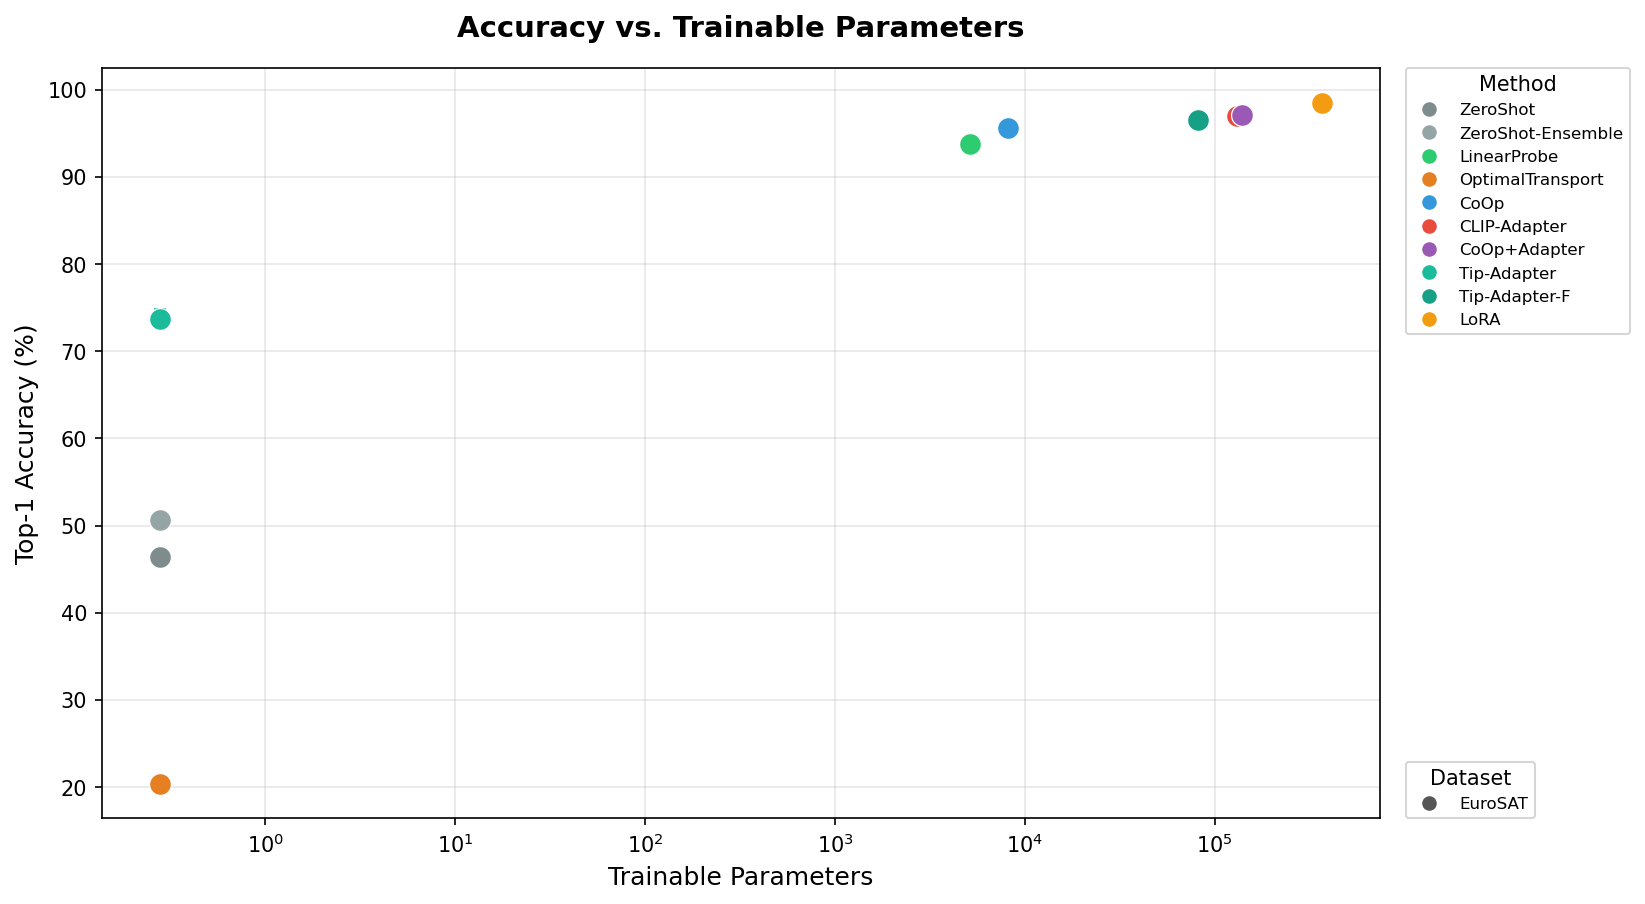
\includegraphics[width=\linewidth]{plots/accuracy_vs_params_unified_eurosat.png}
  \caption{Top-1 accuracy vs.\ trainable parameters on EuroSAT (16-shot),
    logarithmic axis; methods without trainable parameters are drawn at
    the left edge.  Tip-Adapter reaches 74.4\,\% without training, while
    the trained methods, from 5{,}130 to 368{,}640 parameters, all fall
    between 75.9 and 86.3\,\%.}
  \label{fig:acc-vs-params}
\end{figure}

Figure~\ref{fig:acc-vs-params} shows that on EuroSAT the largest step is
bought by labels rather than by parameters.  The training-free
Tip-Adapter, which only caches the features of the 160 support images,
already reaches 74.41\,\%, and the linear probe reaches 78.94\,\% with
5{,}130 parameters, three points above CoOp.  Beyond that point accuracy
is nearly flat in the parameter count: CLIP-Adapter, the joint model and
LoRA land within 0.44 points of each other across a 2.8-fold range of
parameters, and the most accurate method, Tip-Adapter-F, uses fewer
parameters than any of the three.  The ordering is dataset-dependent: on
DTD and Flowers102 CoOp overtakes the linear probe with fewer parameters.

\subsection{Training Cost and Resource Usage}\label{sec:cost}

\begin{table}[t]
\centering
\caption{Wall-clock training time (s), main grid run.  Includes one full
  test-set evaluation per epoch for the methods trained through the shared
  loop, and a single evaluation for Tip-Adapter-F.}
\label{tab:cost}
\small
\begin{tabular}{@{}lrrr@{}}
\toprule
\textbf{Method} & \textbf{EuroSAT} & \textbf{DTD} & \textbf{Flowers102} \\
\midrule
CoOp            & 357  & 285  & 705  \\
CLIP-Adapter    & 356  & 265  & 684  \\
CoOp+Adapter    & 420  & 289  & 713  \\
Tip-Adapter-F   &  44  &  99  & 146  \\
LoRA            & 370  & 290  & 689  \\
\bottomrule
\end{tabular}
\end{table}

Table~\ref{tab:cost} is not pure optimisation cost: the five methods
trained through the shared loop evaluate on the full test set after every
epoch, whereas Tip-Adapter-F is evaluated once.  One evaluation pass takes
about 34\,s on EuroSAT, 18\,s on DTD and 55\,s on Flowers102, so ten of
them account for most of the 265--713\,s reported, and the gap to
Tip-Adapter-F is largely evaluation overhead.  The measurement is also
noisy: repeating the EuroSAT run reproduced every accuracy exactly but
changed the joint model's time from 420 to 343\,s.  We therefore do not
rank the methods by time.

\paragraph{Memory depends on where the gradient flows.}
At evaluation every trainable method sits at 1{,}327--1{,}395\,MB
(Table~\ref{tab:main}), because the frozen backbone dominates.  Training
peaks separate them.  CLIP-Adapter stays at 1{,}339--1{,}420\,MB on all
three datasets, since its backward pass stops at a 512-dimensional MLP;
LoRA needs 2{,}073--2{,}214\,MB to back-propagate through the twelve
visual blocks.  CoOp grows with the number of classes---1{,}424, 2{,}138
and 3{,}213\,MB on EuroSAT, DTD and Flowers102---because every step
back-propagates through the text transformer for all $C$ prompts, and the
joint model follows it within 2\,MB.  Few trainable parameters do not
imply a light training step.

\subsection{Analysis of Optimal Transport Failure}\label{sec:ot-analysis}

We identify three structural reasons for the failure.
\textbf{Misaligned feature spaces:} the output projection is applied to
all tokens, but the contrastive objective only trained the pooled token to
align with text; patch tokens were never optimised for text matching.
\textbf{Uninformative marginals:} uniform weights treat background patches
as important as object-relevant ones, and in satellite imagery the
background dominates the $7 \times 7$ grid.
\textbf{Template-word dominance:} each prompt shares the $[\mathrm{SOS}]$
marker and its template words (``a'', ``satellite'', ``image'', ``of''),
5 of the $\sim$7 non-padding tokens; since the text transformer is causal,
these tokens never attend to the class name and are identical for every
class.  The distance is thus dominated by tokens that carry no class
information, a problem that grows with more descriptive prompts.  On
EuroSAT the result is a near-collapse: 83\,\% of all test images are
assigned to permanent crop land.

\subsection{Ablation Studies}\label{sec:ablations}

\subsubsection{CoOp: Supervision Matters More Than Capacity}\label{sec:coop-ablation}

\begin{table}[t]
\centering
\caption{CoOp ablations on EuroSAT (16-shot, 100 epochs, batch size 32,
  single seed 42).  Each block varies one axis and holds the others at
  $M{=}16$, unified context, $\mathrm{lr}=2\times10^{-3}$, $K{=}16$ (86.63\,\%).
  Best per block in \textbf{bold}.}
\label{tab:coop-ablation}
\footnotesize
\setlength{\tabcolsep}{4pt}
\begin{tabular}{@{}llrr@{}}
\toprule
\textbf{Axis} & \textbf{Setting} & \textbf{Params} & \textbf{Top-1} \\
\midrule
\multirow{6}{*}{Learning rate}
  & $2 \times 10^{-6}$ & 8\,192  & 58.57 \\
  & $2 \times 10^{-5}$ & 8\,192  & 77.20 \\
  & $2 \times 10^{-4}$ & 8\,192  & \textbf{86.83} \\
  & $2 \times 10^{-3}$ & 8\,192  & 86.63 \\
  & $2 \times 10^{-2}$ & 8\,192  & 86.57 \\
  & $2 \times 10^{-1}$ & 8\,192  & 85.89 \\
\midrule
\multirow{3}{*}{Context length}
  & $M = 4$  & 2\,048 & 86.31 \\
  & $M = 8$  & 4\,096 & 86.50 \\
  & $M = 16$ & 8\,192 & \textbf{86.63} \\
\midrule
\multirow{2}{*}{Context type}
  & Unified              &  8\,192 & 86.63 \\
  & Class-specific (CSC) & 81\,920 & \textbf{89.09} \\
\midrule
\multirow{5}{*}{Shots $K$}
  & $K = 1$  & 8\,192 & 69.80 \\
  & $K = 2$  & 8\,192 & 62.43 \\
  & $K = 4$  & 8\,192 & 74.39 \\
  & $K = 8$  & 8\,192 & 82.39 \\
  & $K = 16$ & 8\,192 & \textbf{86.63} \\
\bottomrule
\end{tabular}
\end{table}

Table~\ref{tab:coop-ablation} sweeps four axes of CoOp on EuroSAT, one at
a time.  These runs use 100 epochs and seed 42, so their absolute numbers
are not comparable with Table~\ref{tab:main}.

\paragraph{Learning rate: a step, not a peak.}
At $2\times10^{-6}$ the context barely moves and accuracy stays at
58.6\,\% (77.2\,\% at $2\times10^{-5}$); from $2\times10^{-4}$ upwards,
three orders of magnitude of learning rate land within one point of each
other.  The nominal optimum, $2\times10^{-4}$ (86.83\,\%), sits on a
plateau---every rate up to $2\times10^{-2}$ is within 0.26 points---so we
keep the $2\times10^{-3}$ of the original recipe.  With 8{,}192 parameters
and gradient norms of order $10^{3}$, preliminary runs needed the warmup
epoch for stable training.

\paragraph{Context length and type.}
Quadrupling the context from $M{=}4$ to $M{=}16$ buys 0.32 points: at this
support-set size the prompt's expressiveness is not the bottleneck.
Class-specific context does better, 89.09 against 86.63\,\% ($+2.46$),
the largest effect outside the shot count and the two starved learning
rates.  This agrees with the original study, which finds unified context
better on average and below eight shots, but CSC better on DTD and EuroSAT
at 16 shots~\cite{zhou2022learning}.  The price is ten times the
parameters (81{,}920), still below the CLIP-Adapter budget; whether the
advantage survives the 10-epoch budget of Table~\ref{tab:main} is left
open.

\paragraph{Shots: the axis that moves most.}
Accuracy grows from 69.8\,\% at one shot to 86.6\,\% at sixteen, a
17-point range, while no other axis outside the starved learning rates
moves it by more than 2.5 points---the same pattern as
Figure~\ref{fig:acc-vs-params}.  The one inversion, $K{=}2$ below $K{=}1$,
is an artefact of single-seed sampling: with two images per class, which
images are drawn matters more than how many.

\subsubsection{CLIP-Adapter: Reduction Ratio and Alpha}
\label{sec:adapter-ablation}

\begin{table}[t]
\centering
\caption{CLIP-Adapter ablations on EuroSAT, full training split
  (21{,}600 images), 10 epochs, single seed.  The reduction sweep fixes
  $\alpha{=}0.2$ and the blending sweep fixes $r{=}4$, so the
  configuration $(r{=}4, \alpha{=}0.2)$ appears in both---at 97.11\,\%
  and 97.17\,\%, which measures the run-to-run noise directly.}
\label{tab:adapter-ablation}
\footnotesize
\setlength{\tabcolsep}{4pt}
\begin{tabular}{@{}llrr@{}}
\toprule
\textbf{Axis} & \textbf{Setting} & \textbf{Params} & \textbf{Top-1} \\
\midrule
\multirow{4}{*}{Reduction $r$}
  & $r = 2$  & 262\,912 & \textbf{97.28} \\
  & $r = 4$  & 131\,712 & 97.11 \\
  & $r = 8$  &  66\,112 & 96.81 \\
  & $r = 16$ &  33\,312 & 96.78 \\
\midrule
\multirow{4}{*}{Blending $\alpha$}
  & $\alpha = 0.1$ & 131\,712 & 97.11 \\
  & $\alpha = 0.2$ & 131\,712 & \textbf{97.17} \\
  & $\alpha = 0.5$ & 131\,712 & 96.94 \\
  & $\alpha = 0.8$ & 131\,712 & 97.15 \\
\bottomrule
\end{tabular}
\end{table}

Table~\ref{tab:adapter-ablation} predates the few-shot protocol and uses
the full EuroSAT training split, hence accuracies near 97\,\%.  Both
sweeps are nearly flat.  The configuration $(r{=}4, \alpha{=}0.2)$, run in
both, scored 97.11 and 97.17\,\%: against that 0.06-point noise the
0.23-point $\alpha$ sweep carries no signal, plausibly because the
near-zero initialisation of $W_{\mathrm{up}}$ already does the work
$\alpha$ was introduced for.  The reduction ratio spans 0.50 points,
monotone in capacity, but $r{=}2$ buys its 0.17-point lead with twice the
parameters, so we keep $r{=}4$, $\alpha{=}0.2$ as the better cost
trade-off.

\subsection{Qualitative Analysis}\label{sec:qualitative}

\begin{figure*}[!tp]
  \centering
  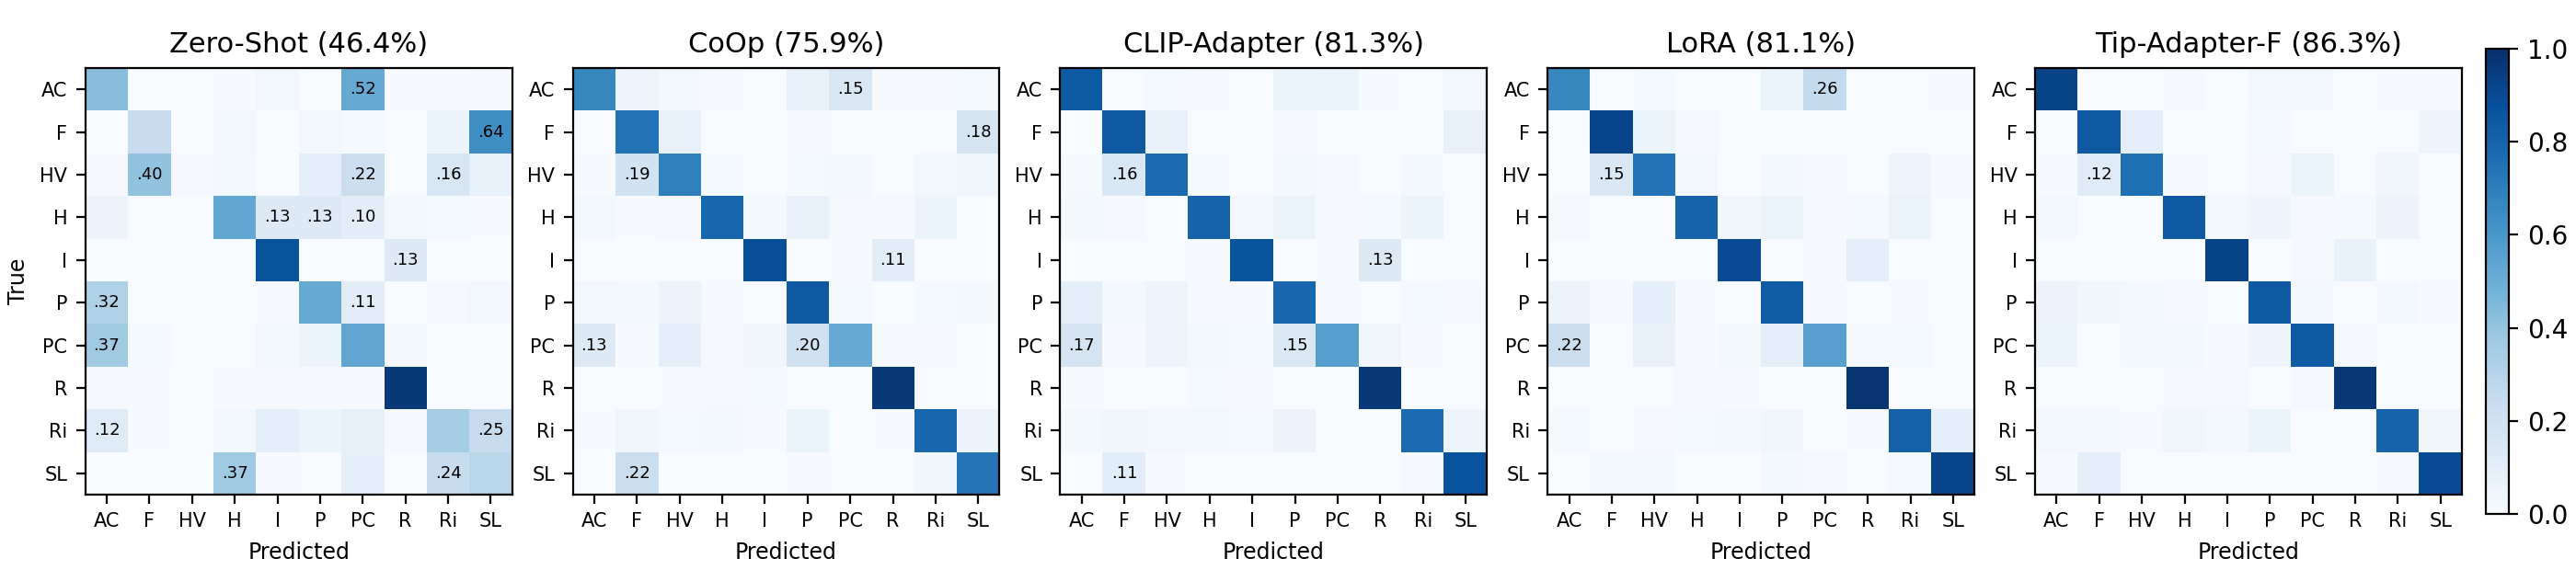
\includegraphics[width=\textwidth]{plots/confusion_matrices_compact_eurosat.png}\\[2pt]
  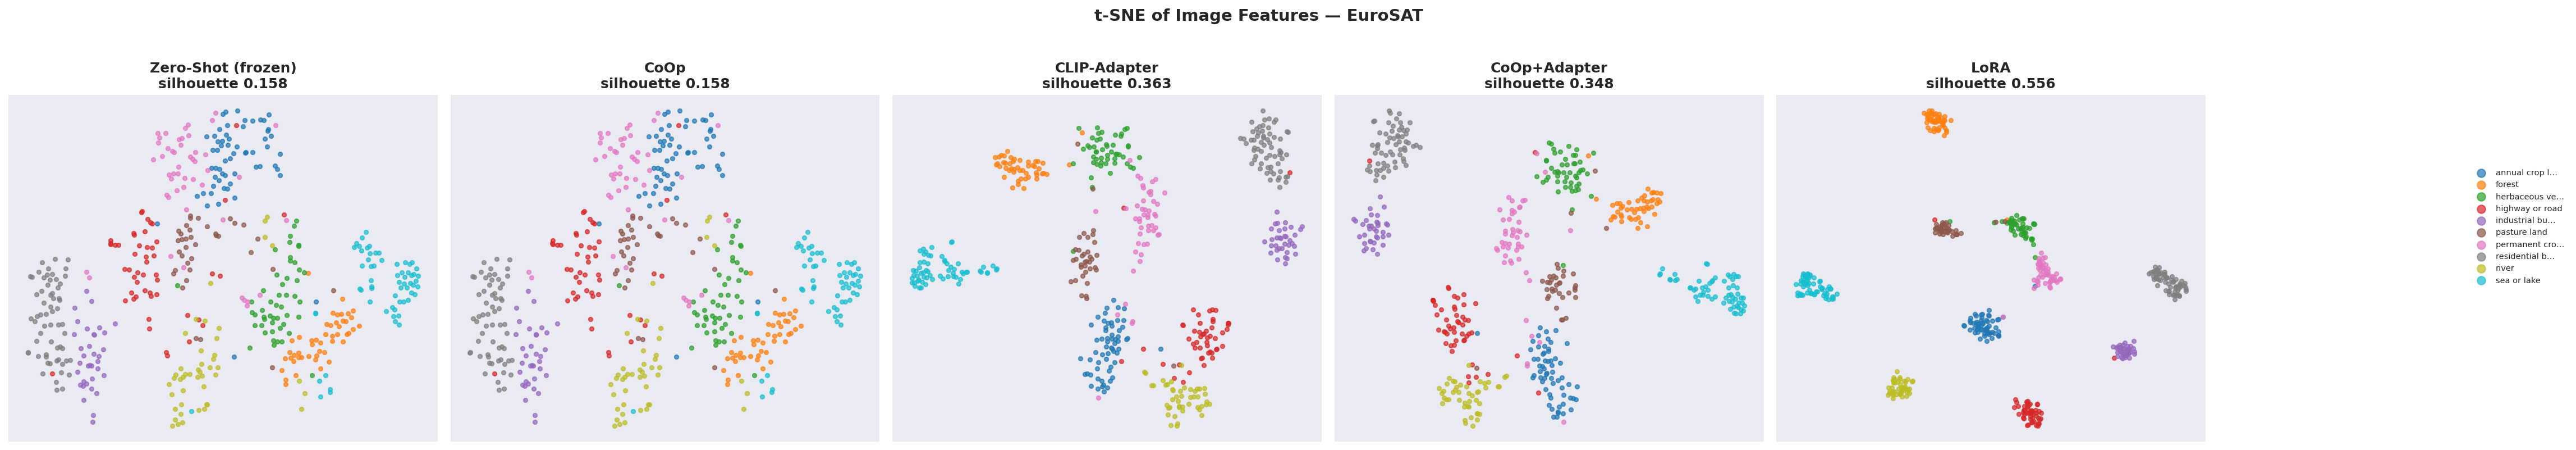
\includegraphics[width=\textwidth]{plots/tsne_features_eurosat.png}
  \caption{EuroSAT, 16-shot.  \emph{Top:} row-normalised confusion
    matrices, off-diagonal entries $\geq 0.10$ annotated (AC annual crop,
    F forest, HV herbaceous vegetation, H highway, I industrial, P pasture,
    PC permanent crop, R residential, Ri river, SL sea or lake).
    \emph{Bottom:} t-SNE of 500 test-image features with silhouette scores
    computed in the original space; CoOp leaves the image space unchanged
    by design.}
  \label{fig:qualitative}
\end{figure*}

Figure~\ref{fig:qualitative} (top) shows that zero-shot CLIP confuses whole
groups of land-use classes: 64\,\% of forest images become sea or lake,
and 52\,\% of annual crop becomes permanent crop.  After adaptation the
residual errors concentrate in two groups of visually related classes,
vegetated or water surfaces and agricultural land, with a method-dependent
emphasis: CoOp's largest confusion is sea or lake $\to$ forest (0.22),
CLIP-Adapter's permanent $\to$ annual crop (0.17), LoRA's annual $\to$
permanent crop (0.26), while Tip-Adapter-F keeps every off-diagonal entry
at or below 0.12.

The t-SNE panels (bottom) are computed on image features.  CoOp's is
identical to zero-shot (silhouette 0.158) by construction: CoOp never
touches the image encoder and gains its 29.5 points by moving the text
prototypes within a fixed image space.  CLIP-Adapter and the joint model
barely change the cluster structure (0.168 and 0.167) despite adding
5.4--5.7 points over CoOp, which suggests that their gain, too, comes less
from tighter clusters than from bringing image features closer to the
text prototypes.  LoRA, which adapts the encoder from the inside, is the
only method that visibly separates the classes (0.245), yet it is no more
accurate than the adapter: separability of the image features and
alignment with the text prototypes are different properties.


\section{Conclusion}\label{sec:conclusion}

We compared ten methods---seven families of parameter-efficient
adaptation, two zero-shot baselines and an exploratory Optimal Transport
variant---on three benchmarks with a common frozen ViT-B/32 backbone.
Four findings stand out.  \textbf{Labels buy more than parameters}: once
16 images per class (10 on Flowers102) are available, the parameter count
predicts accuracy poorly.  On EuroSAT the training-free Tip-Adapter and a
5{,}130-parameter linear probe close 70\,\% and 82\,\% of the gap between
zero-shot CLIP and the best method, and within CoOp the shot count moves
accuracy far more than context length or type.  \textbf{Extreme parameter
efficiency is nonetheless achievable where the text side matters}: on DTD
and Flowers102, CoOp's 16 context vectors (0.005\,\% of the backbone)
close 90\,\% and 76\,\% of that gap and beat the linear probe with fewer
parameters.  \textbf{Joint text--vision adaptation yields marginal gains}:
the combined model lands within 0.33 points of the better half on all
three datasets ($+0.33$, $-0.16$, $-0.23$), suggesting overlapping
contributions, and reaching even that parity required the adapter's
optimiser recipe rather than CoOp's.  \textbf{Token-level Optimal Transport
fails without careful engineering}, for the structural reasons of
Section~\ref{sec:ot-analysis}.  Two observations qualify these results:
Tip-Adapter-F is the most accurate method on two datasets out of three,
but its parameter count grows with the number of classes; and few
trainable parameters do not mean a light training step, since CoOp's
training memory grows from 1.4 to 3.2\,GB with $C$ while the adapter's
stays near 1.4\,GB.  In practice: start with prompt ensembling, which is
free; with labels, try Tip-Adapter and a linear probe first; move to CoOp
or CLIP-Adapter where those fall behind, as on DTD and Flowers102.

\paragraph{Limitations.}
There is \textbf{no validation split}: per-epoch accuracy is measured on
the test set, and the ablations behind our hyperparameter choices were
scored on it too, as is common in the few-shot CLIP literature, so our
accuracies are optimistic (we report the final epoch, not the best).
Every number comes from a \textbf{single seed} (0 for the main grid, 42
for the CoOp ablations); the only spread we measure, 0.06 points between
two runs of one adapter configuration, is smaller than the effects we
discuss, but differences of a few tenths are not meaningful, and
wall-clock times are noisier still.  The \textbf{ablations follow
different protocols} from the main grid and from each other, both on
EuroSAT only.  We use a single backbone with \textbf{LAION-2B weights}
rather than the OpenAI checkpoint, never ViT-L/14, and apply no data
augmentation, unlike the original CoOp and CLIP-Adapter papers.

\paragraph{Future work.}
A held-out validation split, standard augmentations and a ViT-L/14 repeat
would remove those limitations.  The Optimal Transport failure is
actionable---attention-derived marginals and class-name-only text
tokens---and conditional context generation~\cite{zhou2022conditional},
which makes the context a function of the image rather than of the class,
is the natural next step after the class-specific result.


\section{Contributions}\label{sec:contributions}

\noindent\textbf{Mattia} focused on the core infrastructure, implementing \texttt{BaseCLIPWrapper} (\texttt{base\_model.py}) to expose the virtual \texttt{get\_image\_features()} and \texttt{get\_text\_features()} overridden later by the other members, together with the shared \texttt{predict()} method and patch-level extraction for Optimal Transport. Furthermore, the unified evaluation and training engine (\texttt{engine.py}), featuring a model-agnostic \texttt{evaluate()} loop (Top-1/5, GPU tracking, W\&B) and a generic \texttt{train()} function with per-module optimizer groups, cosine annealing, and a one-epoch learning-rate warmup. Additional development included the dataset loaders (\texttt{dataset.py}) for EuroSAT, DTD, and Flowers102 with per-dataset prompt templates, the seeded per-class K-shot sampling protocol (\texttt{few\_shot.py}), and the zero-shot, prompt ensembling, and linear baselines (\texttt{baselines.py}). Finally, the Optimal Transport module (\texttt{optimal\_transport.py}) and the \texttt{run\_all.py} script were developed to enforce the fair-comparison protocol (matched support set, matched epoch budget, multi-seed aggregation) and generate comparative figures.

\medskip

\noindent\textbf{Marco} managed the vision-side adaptation, authoring the \texttt{VisionAdapterModule} (\texttt{clip\_adapter.py}) to provide a bottleneck MLP (down-projection, ReLU, near-zero-initialized up-projection) with residual blending \(f = \alpha\,\text{MLP}(f) + (1{-}\alpha)\,f\), supporting both fixed and learnable \(\alpha\) parameters. Work included subclassing \texttt{BaseCLIPWrapper} into \texttt{CLIPAdapterModel} to override \texttt{get\_image\_features()}, and implementing the training-free \texttt{TipAdapterModel} with a key--value cache built from a K-shot support set, alongside \texttt{Tip-Adapter-F} for cache key fine-tuning as \texttt{nn.Parameter}. Additionally, the \texttt{LinearLoRA} module and \texttt{VisionLoRAModel} were developed to inject LoRA into the vision transformer's MLP blocks (\texttt{c\_fc} and \texttt{c\_proj}). Finally, the adapter experiment script (\texttt{clip\_adapter\_experiments.py}) and the execution of the full experimental grid on a local machine, generating the ablations of Table~\ref{tab:adapter-ablation} (reduction ratio and alpha sweep) and graphs included in this report.

\medskip

\noindent\textbf{Carlo} was responsible for the text-side adaptation. He
implemented the \texttt{PromptLearner} module (\texttt{coop.py}): learnable
context vectors \texttt{ctx} as an \texttt{nn.Parameter}, frozen
\texttt{[SOS]} prefix and class-name suffix buffers obtained through a
placeholder tokenization, and both Unified $(M, D)$ and Class-Specific
$(C, M, D)$ context. \texttt{CoOpModel} overrides
\texttt{get\_text\_features()} with a manual text-encoder forward pass that
starts from embeddings rather than token ids, deliberately without
\texttt{@torch.no\_grad()} so that gradients reach the context. He wrote the
seeded class-balanced K-shot sampler (\texttt{few\_shot.py}) and the joint
\texttt{CoOpAdapterModel} (\texttt{coop\_adapter.py}), which sidesteps the
MRO conflict of multiple inheritance by subclassing only
\texttt{BaseCLIPWrapper} and borrowing the two feature methods, and exposes
per-module optimizer groups through \texttt{trainable\_param\_groups()}.
He wrote \texttt{coop\_experiments.py} and ran the ablations of
Table~\ref{tab:coop-ablation}.


{\small
\bibliographystyle{ieeetr}
\bibliography{references}
}

\end{document}
